%=====================================================================
\chapter{Ergebnisse}
\label{sec:Ergebnisse}
%=====================================================================
TODO

\section{Baseline}
TODO
%
%
\section{Autoencoder}
Dieses Kaptil stellt zuerst einmal das Verhalten eines VAE beispielhaft an dem MNIST Datensatz dar. MNIST ist ein Datensatz aus Bildern von handgeschriebenen Zahlen zwischen Null und Neun. Jedes Bild hat dabei 28x28 Pixel. Der Datensatz beinhaltet 60000 Bildern f�r das Training und 10000 f�r die Evaluation. Anschlie�end werden die Ergebnisse der Dataaugmentation f�r den Datensatz dr Spektorgramme pr�sentiert. Dar�ber hinaus wird gezeigt, welchen Einfluss die Dataaugmentation auf das Klassifikationsergebnis hat.\\
\\
%
Das Encodernetz $Q$ soll die Eingangsdaten $X$ in einen Zwischenraum $z$ mappen. F�r den MNIST Datensatz wird eine zweidimensionale Gausverteilung gew�hlt um, sodass $z\sim N(0,I)$. Nach dem Training des VAE l�sst sich der Latentraum $Q(z|X)$ darstellen wie in Abbildung x gezeigt. Jeder Punkt in Abbildung X ist dabei die Repr�sentation $z_i$ des zugeh�rigen Eingangsbild $X_i$. Abbildung X zeigt, dass der gelernte Latentraum einer Gausverteilung $N(0,I)$ entspricht. Auch ist zu erkennen, dass sich Samples mit gleichem Label zu Clustern formieren. So k�nnen sp�ter durch abtasten der Verteilung $P(z)$ Bilder aus den verschiedenen Klassen generiert werden.\\
Anschlie�end k�nnen die encodeden Bilder vom Decoder $P$ wieder rekonstruiert werden. In diesem Fall soll der VAE Bilder von handgeschriebenen Zahlen encoden und anschlie�end rekonstruieren. Dieses Verhalten ist in Abbildung X dargestellt. Die obere Zeile beinhaltet beispielhafte Zahlen von Null bis Neun aus dem MNIST Datensatz. Diese werden durch den VAE geschickt und dabei encoded. Die rekonstruierten Bilder sind in der unteren Zeile dargstellt. Es ist zu erkennen das der VAE in den meisten F�llen die Ursprungszahl wiederherstellen kann. Allerdings hat der VAE bei manchen Ziffern deutlich mehr Probleme die Form zu rekonstuieren. Dabei ist auffallend, dass Ziffern dazu tendieren die Form einen anderen Zahl anzunehmen. Der Gurnd daf�r ist, dass der Latentraum eine continuierliche Verteilung repr�sentiert und somit die Grenzen zwischen den Clustern flie�end sind. Beispielsweise die Ziffer 3 wird hier als Ziffer 5 rekonstuiert. Betrachtet man den Latentraum bzw. den Manifold der generierten Bilder ist zu erkennen, dass sich die Cluster der Ziffern 3,5 und 8 alle in der Mitte sammeln und sich teilweise �berlagern. Dies kann dazu f�hren, dass Ziffern aus diesem Bereich als andere Zahl rekonstruier werden.\\
Durch Abtasten des Latentraum k�nnen neue Samples aus der gelernten Verteilung gezogen werden. Diese k�nnen als Input f�r den Decoder $P$ verwendet werden um so neue ungesehene Bilder zu generieren. Hierzu wird die Gaussverteilung in x- und y-Richtung abgetastet. Abbildung X zeigt den Verlauf der rekonstuierten Bilder. Es ist zu erkennen, dass durch Samples aus den verschiedenen Clustern ein �bergang zwischen den verschieden Ziffern entsteht. Ein Hauptproblem des VAE ist die Eigenschaft, dass sowohl die rekosntruierten als auch die generierten Bild verschwommen sind und nicht die scharfen Konturen der Orginalbilder aufweisen. Dies liegt an der Beschr�nkung des Latentraums auf eine simplen zweidimensionale Gaussverteilung. Diese Verteilung reicht nicht aus um alle Aspekte der Eingangsdaten abzubilden. H�herdimensionale Verteilungen erm�glichen daher vrbesserte Rekonstrukitionseigenschaften. Allerdings wird dadurch auch der Samplingprozess zu generierung neuer Daten erschwert, da es deutlich komplexer ist solch eine Verteilung abzutasten.\\
\\
%
Tabelle \ref{VAEencArchitecturMNIST} und \ref{VAEdecArchitecturMNIST} zeigen die Encoder und Decoder Architektur des VAE f�r den MNIST Datensatz. Der Encoder besitzt zu Begin vier Convolutional Ebenen mit steigender Filteranzahl von 32, 64 und 128. Zus�tlich wird in Striding von $2x2$, wodurch der Input gedownsampled wird um den Rechenaufwand zu verringern. In der vierten Conv Ebene wird kein Striding mehr angewandt. Als Aktivierungsfunktion wird in allen Conv Ebenen die ReLU Funktion verwendet. Auf die Conv Ebenen folgt jeweils eine Dropout Ebene um die Generalisierung zu erh�hen. Das Resultat der Conv Ebenen sind $4\times4\times128$ Feature Maps. Diese werden in der Flatten Ebene zu einem Vektor umgeformt und durch eine vollverkettete Ebene mit 512 Units geschickt. Zuletzt muss der Latentraum $z$ erzeugt werden. Dieses wird wie in Kapitel X beschreiben als Gausverteilung definiert. Eine Gausverteilung wird �ber zwei Parameter den Erwartungswert $\mu(X)$ und die Varianz $\sigma^2(X)$ beschreiben. Dazu wird das Netz an dieser Stelle aufgespaltet indem zwei vollverkettete Ebenen parallel verwendet werden. Das Netz besitz somit zwei Ausgangsebenen. Diese Ebenen besitzen jeweils zwei Hidden Units um so eine zweidimensionale Gaussverteilung zu erzeugen.\\  
\\
Den Encoder soll Samples, gezogen aus dem Latentraum $z$ wieder auf die urspr�ngliche Eingabe zur�ck mappen. Dazu besitzt der Encoder erste Ebene eine Sampling Funktion, welche aus dem Input $\mu(X)$ und $\sigma^2(X)$ den Latentraum $z=\mu(X)+\Sigma^{\frac{1}{2}}(X)\epsilon$ erzeugt, sodass dieser differenzierbar bleibt. Die Implementierung wird in Algorithmus \ref{Sampling} gezeigt. Dabei wurde die Varianz als log-Varianz modelliert um ein numerisch stabileres Verhalten zum erzielen.\\
%
Nach der Sampling Ebene besitzt der Decoder zwei vollverkettete Ebenen mit 512 und 1152 Hidden Units. Um daraus wieder ein zweidimensionales Bild zu erhalten wird eine Reshape Ebene eingesetzt welche eine $3\times3\times128$ Feature Map erzeugt. Anschlie�end werden drei Convolution Transposed Ebenen verwednet mit Kernel Gr��e $3\times3$ und Striding $2\times2$. Die Conv Transposed mit Striding sorgt daf�r, dass der Input wider geupsamplet wird um so die Ursprungsgr��e der Daten wieder zu erlangen. Zus�tzlich wird hier eine BatchNorm verwendet.
%
%
%
\begin{comment}
\begin{tikzpicture}
\begin{axis}[enlargelimits=false,colorbar,xmin=-6,xmax=6,ymin=-6,ymax=6]
\addplot+[only marks,scatter,scatter src=explicit] table[x=x,y=y,meta=label] {latentSpace.txt};
\end{axis}
\end{tikzpicture}
%
%
%
\begin{figure}[ht]
	\centering
	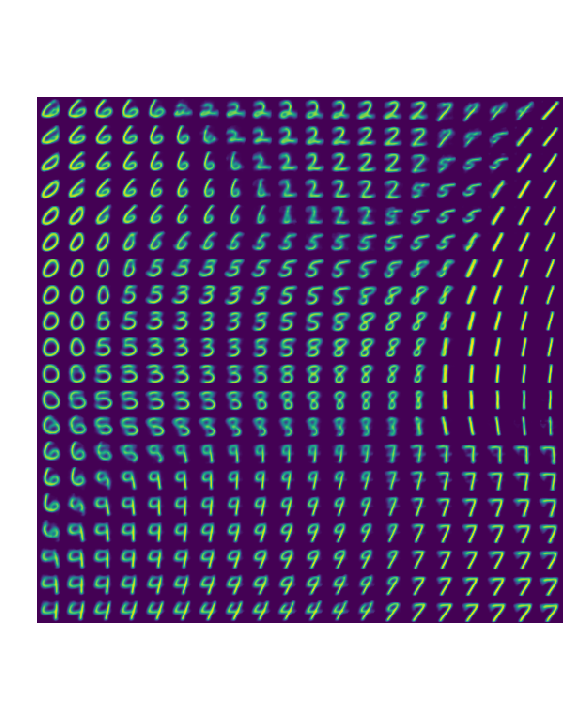
\includegraphics[width=0.66\textwidth]{generationOverLatent.png}
	\caption{MNIST Manifold}
	\label{MNISTmanifold}
\end{figure}
%
%
%
\begin{figure}%[ht]
  \centering
  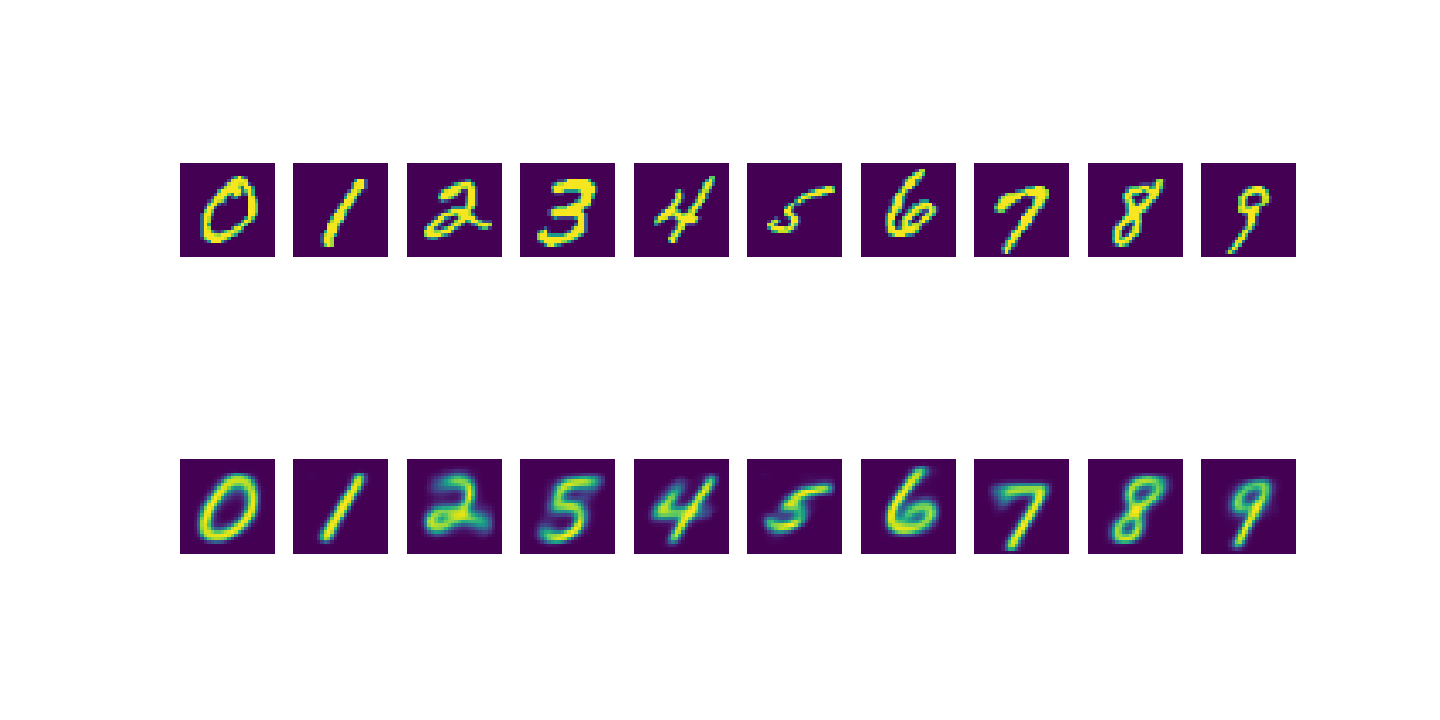
\includegraphics[width=.8\linewidth]{MNISTrecon0-9.png}
  \caption{Orginal und rekonstruierte Bilder}
  \label{MNISTrecon0-9}
\end{figure}
%
%
%
\begin{table}
\begin{tabular}{c c c c c c c}
\toprule
Operation&Kernel&Strides&Feature maps&BN?&Dropout&Nonlinarity\\
\midrule
Input&N/A&N/A&N/A&N/A&N/A&N/A\\
Convolution&3x3&2x2&32&\ding{55}&0.3&ReLU\\
Convolution&3x3&2x2&64&\ding{55}&0.3&ReLU\\
Convolution&3x3&2x2&128&\ding{55}&0.3&ReLU\\
Convolution&3x3&1x1&128&\ding{55}&0.3&ReLU\\
Flatten&N/A&N/A&N/A&\ding{55}&\ding{55}&N/A\\
Dense&N/A&N/A&512&\ding{55}&\ding{55}&ReLU\\
Dense $\mu(X)$&N/A&N/A&2&\ding{55}&\ding{55}&Linear\\
Dense $\sigma^2(X)$&N/A&N/A&2&\ding{55}&\ding{55}&Linear\\
\toprule
\end{tabular}
\caption{Encoder Architektur des VAE f�r den MNIST Datensatz}
\label{VAEencArchitecturMNIST}
\end{table}
%
%
\begin{table}
\begin{tabular}{c c c c c c c}
\toprule
Operation&Kernel&Strides&Feature maps&BN?&Dropout&Nonlinarity\\
\midrule
Input $\mu(X)$&N/A&N/A&N/A&N/A&N/A&N/A\\
Input $\sigma^2(X)$&N/A&N/A&N/A&N/A&N/A&N/A\\
Sampling&N/A&N/A&N/A&\ding{55}&\ding{55}&N/A\\
Dense&N/A&N/A&512&\ding{55}&\ding{55}&ReLU\\
Dense&N/A&N/A&1152&\ding{55}&\ding{55}&ReLU\\
Reshape&N/A&N/A&N/A&N/A&N/A&N/A\\
ConvTransposed&3x3&2x2&128&\ding{51}&0.3&Leaky ReLU\\
ConvTransposed&3x3&2x2&64&\ding{51}&0.3&Leaky ReLU\\
ConvTransposed&3x3&2x2&32&\ding{51}&0.3&Leaky ReLU\\
ConvTransposed&3x3&1x1&1&\ding{55}&0.3&Sigmoid\\
\toprule
\end{tabular}
\caption{Decoder Architektur des VAE f�r den MNIST Datensatz}
\label{VAEdecArchitecturMNIST}
\end{table}
%
%
%
\begin{algorithm}
\caption{Sampling}
\begin{algorithmic}
\REQUIRE $\mu(X),~\sigma^2(X)$
%\ENSURE $abc$
\STATE $\epsilon \sim \mathcal{N}(0,I)$
\STATE $z = \mu(X)+e^{\frac{\mathrm{log}(\sigma)}{2}}(X)\epsilon$
\end{algorithmic}
\label{Sampling}
\end{algorithm}
\end{comment}
%
%
https://arxiv.org/pdf/1406.5298.pdf\\
%
%
\section{GAN}
TODO
\section{Attak-Defence}
TODO